\section{LQR1}
With default Q and R
\begin{figure}[H]
	\centering
	\begin{subfigure}[b]{0.45\textwidth}
		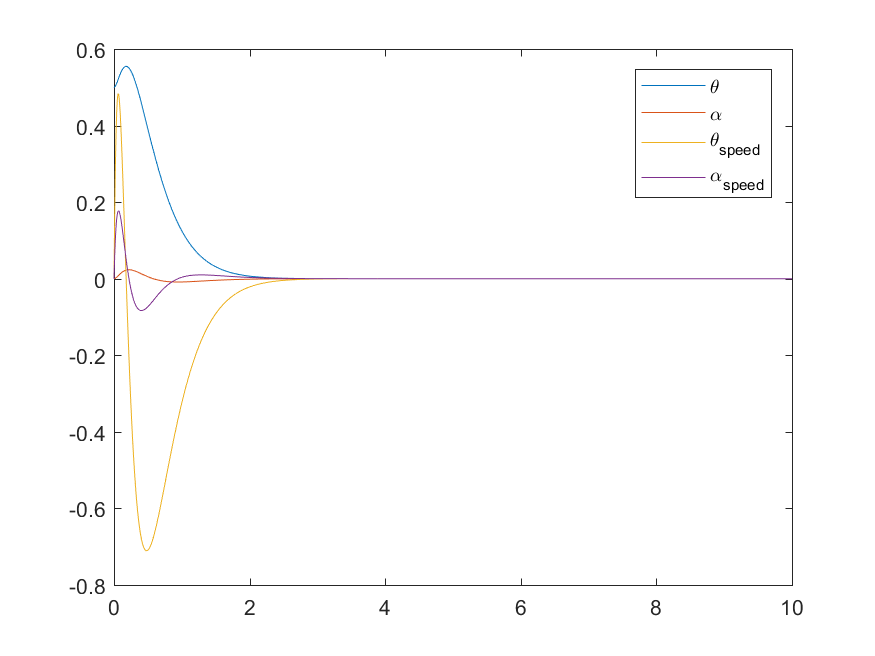
\includegraphics[width=\textwidth]{./part2_LQR1/default_QR_states.png}
		\caption{plot of the states in function of time}
	\end{subfigure}
	\begin{subfigure}[b]{0.45\textwidth}
		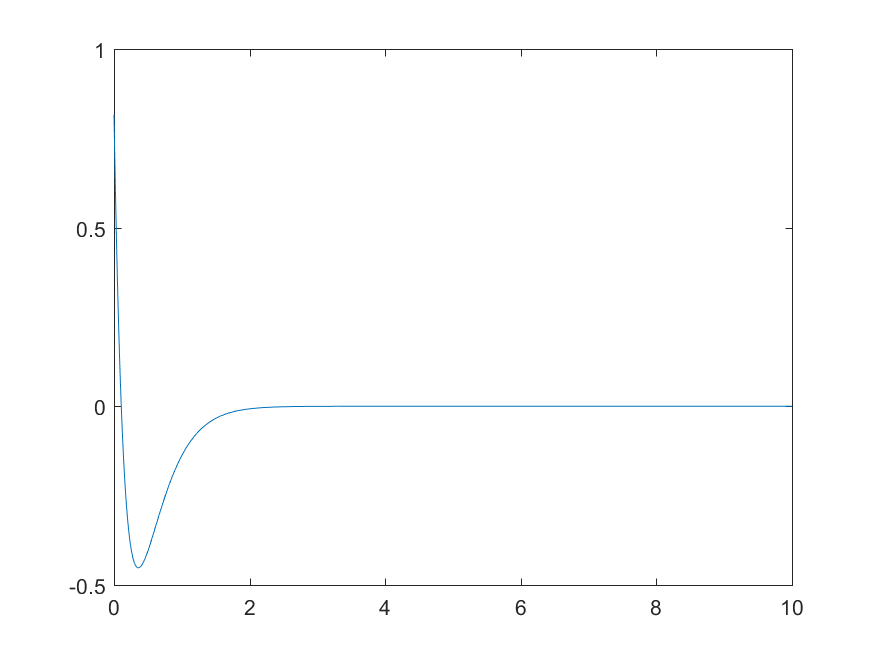
\includegraphics[width=\textwidth]{./part2_LQR1/default_QR_inputs.png}
		\caption{plot of the input signal in function of time}
	\end{subfigure}
	\caption{RIP with 0.5 as start position and a desired position 0}
\end{figure}

\begin{figure}[H]
	\centering
	\begin{subfigure}[b]{0.45\textwidth}
		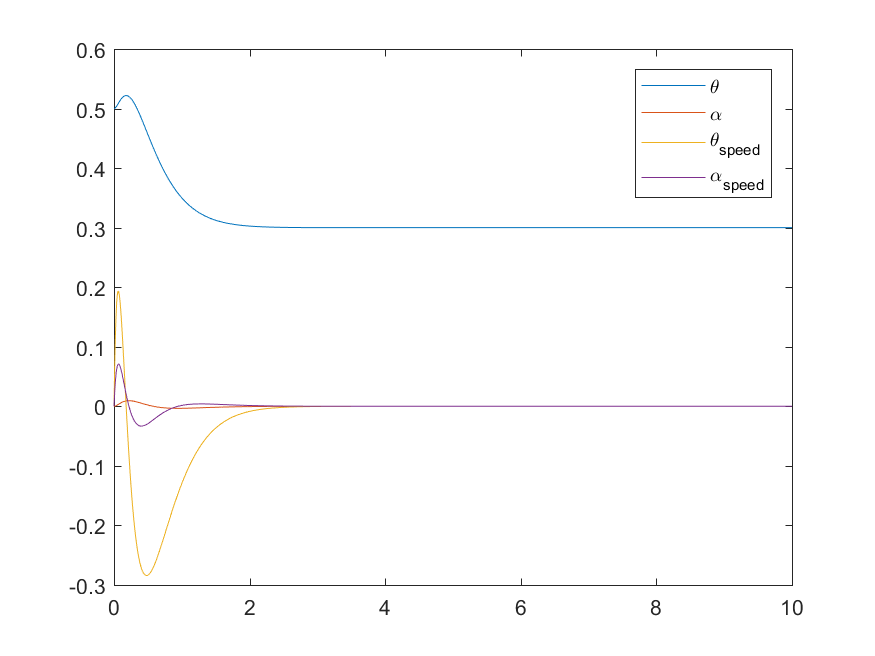
\includegraphics[width=\textwidth]{./part2_LQR1/default_QR_with_desired_states.png}
		\caption{plot of the states in function of time}
	\end{subfigure}
	\begin{subfigure}[b]{0.45\textwidth}
		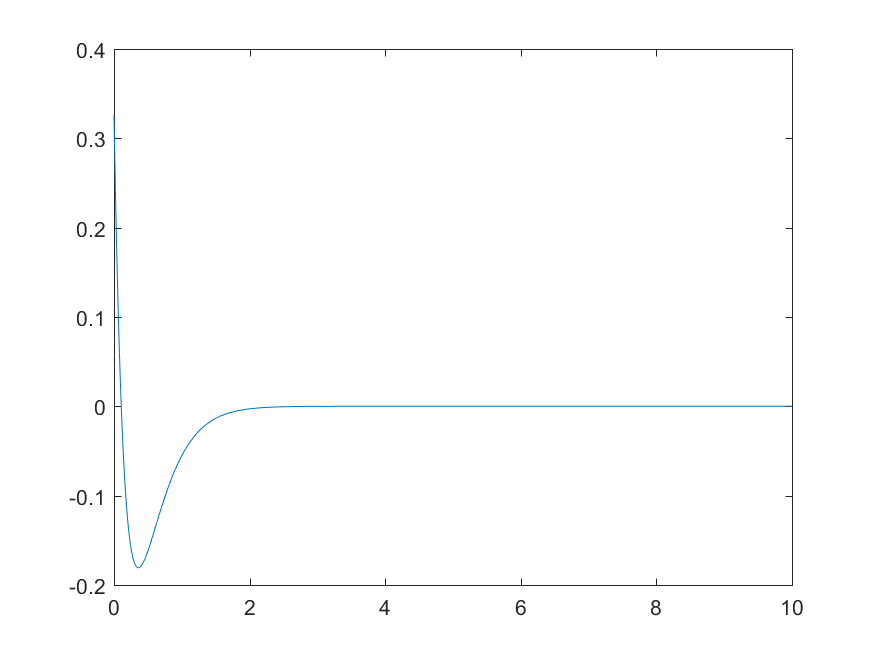
\includegraphics[width=\textwidth]{./part2_LQR1/default_QR_with_desired_inputs.png}
		\caption{plot of the input signal in function of time}
	\end{subfigure}
	\caption{RIP with 0.5 as start position and a desired position 0.3}
\end{figure}